\section{Horizontal RGB Mirroring and Hand-Side Robustness}\label{app:mirror}
\subsection{Question, Motivation and Source Population}
This follow-up asks whether adding horizontal RGB mirrors of training images changes precision and F1 on a controlled mixture of original and mirrored held-out images. It is separate from the primary comparison of interpretable feature representations. Left-handed fingerspelling is legitimate; \href{https://www.lifeprint.com/asl101/pages-layout/lefthandedsigners.htm}{Vicars (ASL University)} describes its mirrored relationship with right-handed signing. Here the original static A--Z labels are retained under horizontal reflection. J and Z are static dataset poses, not tests of their movement.

The historical 78,000-image manifest contains 60,251 accepted single-hand detections: 57,424 are labelled Right by MediaPipe (95.31\%) and 2,827 Left (4.69\%). The remaining 17,749 have no accepted single-hand estimate. These are detector predictions about depicted hands, not verified annotations or evidence of the signer's preferred hand. The dataset is therefore predominantly detector-labelled Right among accepted images; the prevalence over all source images is not known.

\subsection{Independent Pixel Reflection and Detection}
All 78,000 originals and their horizontal RGB reflections are processed afresh. Reflection reverses pixel columns at unchanged resolution, with no interpolation, image rotation, finger-index permutation or label substitution. The same MediaPipe model hash and version, IMAGE mode, maximum two hands, and detection/presence thresholds 0.5/0.5 are used in both views. Each image is detected independently. Image landmarks, world landmarks and handedness are taken from its own detector result. This avoids assuming that the detector is exactly reflection-equivariant or that changing a handedness string changes the hand geometry.

Both views use the existing live encoder: 190 normalized image-landmark distances, 630 axis-direction values and 15 world-joint measurements (835 inputs). Exactly one hand must pass the geometric and finite-descriptor checks. In a purely geometric reflection control, image $x$ becomes $1-x$, world $x$ changes sign, and handedness swaps while anatomical landmark IDs stay fixed. Distances and interior angles are preserved; axis-$x$ direction cosines change sign. Unit tests check that relationship, but the actual experiment reruns detection on reflected pixels rather than substituting ideal reflected features.

Fresh detection accepts \MirrorOriginalAccepted\ originals, \MirrorFlippedAccepted\ mirrors and \MirrorPairedAccepted\ source pairs with both views accepted. These fresh results have their own provenance; the earlier 97.748\% historical-cache score is not the baseline for attributing a mirror effect.

\subsection{Training and Fixed Evaluation}
The five historical filename-block partitions are applied to all source IDs, including earlier rejected images. Every derivative inherits its original source group, so no reflected sibling can occur across the training/evaluation boundary. The groups are not verified people or sessions. For each fold, the baseline trains on freshly accepted originals from fitting groups. The candidate adds a successfully detected mirror only for those same fitting sources. Originals whose mirror fails remain; mirror-only recoveries do not enlarge the source population. This separates reflected presentation from adding new source images.

Each source contributes total fitting weight one: 0.5 per view when both are available, otherwise one for its original. Median imputation and angle scaling are fitted on original fitting rows and shared by the two arms. The SVM uses $C=10$ with its original-fit resolved RBF gamma and balanced class weights; the candidate therefore does not gain a different kernel bandwidth or class prior through duplication. LightGBM retains 100 trees, 31 leaves, learning rate 0.1, minimum child samples 20 and seed 42. Its row-count-dependent tree constraints can still respond to augmentation. No mirror parameters or hyperparameters are tuned on held-out outcomes.

Three presentations use the same held-out sources: originals; their RGB mirrors; and a fixed random mix containing one view per source. Seed 20261106 selects half the sources within each letter/fold for reflection, giving \MirrorMixOriginal\ originals and \MirrorMixFlipped\ mirrors. Both models see identical selected images. Selection occurs before model predictions and is not conditioned on detection success. The mix contains \MirrorMixedAccepted\ accepted detections, of which the detector labels \MirrorMixedLeft\ Left (\MirrorMixedLeftPercent\%) and \MirrorMixedRight\ Right (\MirrorMixedRightPercent\%). Equal reflection frequency is not the same as exactly equal true hand prevalence.

All-attempt results retain failed detections as no prediction (\texttt{?}). Macro-precision, recall and F1 average the 26 letter scores, with undefined scores set to zero. No prediction contributes a false negative for its true letter, so it reduces recall/F1 but adds no false positive. Accepted-only results use the same accepted images for both classifiers. A further paired-both-accepted subset permits comparison of presentations without changing the source population. Source pairs are never treated as independent people or used to claim twice the effective sample size.

\begin{table}[h]
\centering\small
\caption{Pooled held-out results over all 78,000 attempted sources per presentation. No-prediction failures are retained. P denotes macro-precision; each source has exactly one selected view in the balanced mix.}
\begin{tabular}{lllrrr}\toprule
Learner & Presentation & Training & Acc. (\%) & P (\%) & Macro-F1\\\midrule
\tableinput mirror_detail_rows.tex
\bottomrule\end{tabular}
\end{table}

\begin{table}[h]
\centering\small
\caption{Conditional results on successful detection in each presentation. The two training arms use the same accepted evaluation images; the accepted subset can differ between presentations.}
\begin{tabular}{lllrrr}\toprule
Learner & Presentation & Training & Accepted & P (\%) & Macro-F1\\\midrule
\tableinput mirror_conditional_rows.tex
\bottomrule\end{tabular}
\end{table}

\subsection{Interpretation and Limits}
For SVM, balanced-mix macro-precision changes from \MirrorMixPrecisionBase\% to \MirrorMixPrecisionAug\%, and macro-F1 from \MirrorMixFoneBase\ to \MirrorMixFoneAug, with a net correct-count change of \MirrorMixNet. On originals the F1 comparison is \MirrorOrigFoneBase\ versus \MirrorOrigFoneAug\ (net \MirrorOrigNet); on mirrors it is \MirrorFlipFoneBase\ versus \MirrorFlipFoneAug\ (net \MirrorFlipNet). The LightGBM balanced-mix changes are \MirrorLgbPrecisionDelta\ percentage points in precision and \MirrorLgbFoneDelta\ in F1. Read the joint outcomes rather than selecting only the favourable presentation or letters.

The test mix estimates this artificial presentation distribution, not left/right prevalence in actual use. Original/mirror pairs share identity, pose and background. Pixel reflection cannot create independent left-handed signers, natural variations of signing, new viewpoints or new illumination. The detector's handedness labels are not ground truth. No separate left-handed cohort or independent final classification test is available, and this family of filename-block folds has informed earlier development. Scores and fold differences are descriptive, not confirmatory population-level inference. Results of this augmentation do not establish that the explicit hand features themselves improve recognition.

\begin{figure}[h]
\centering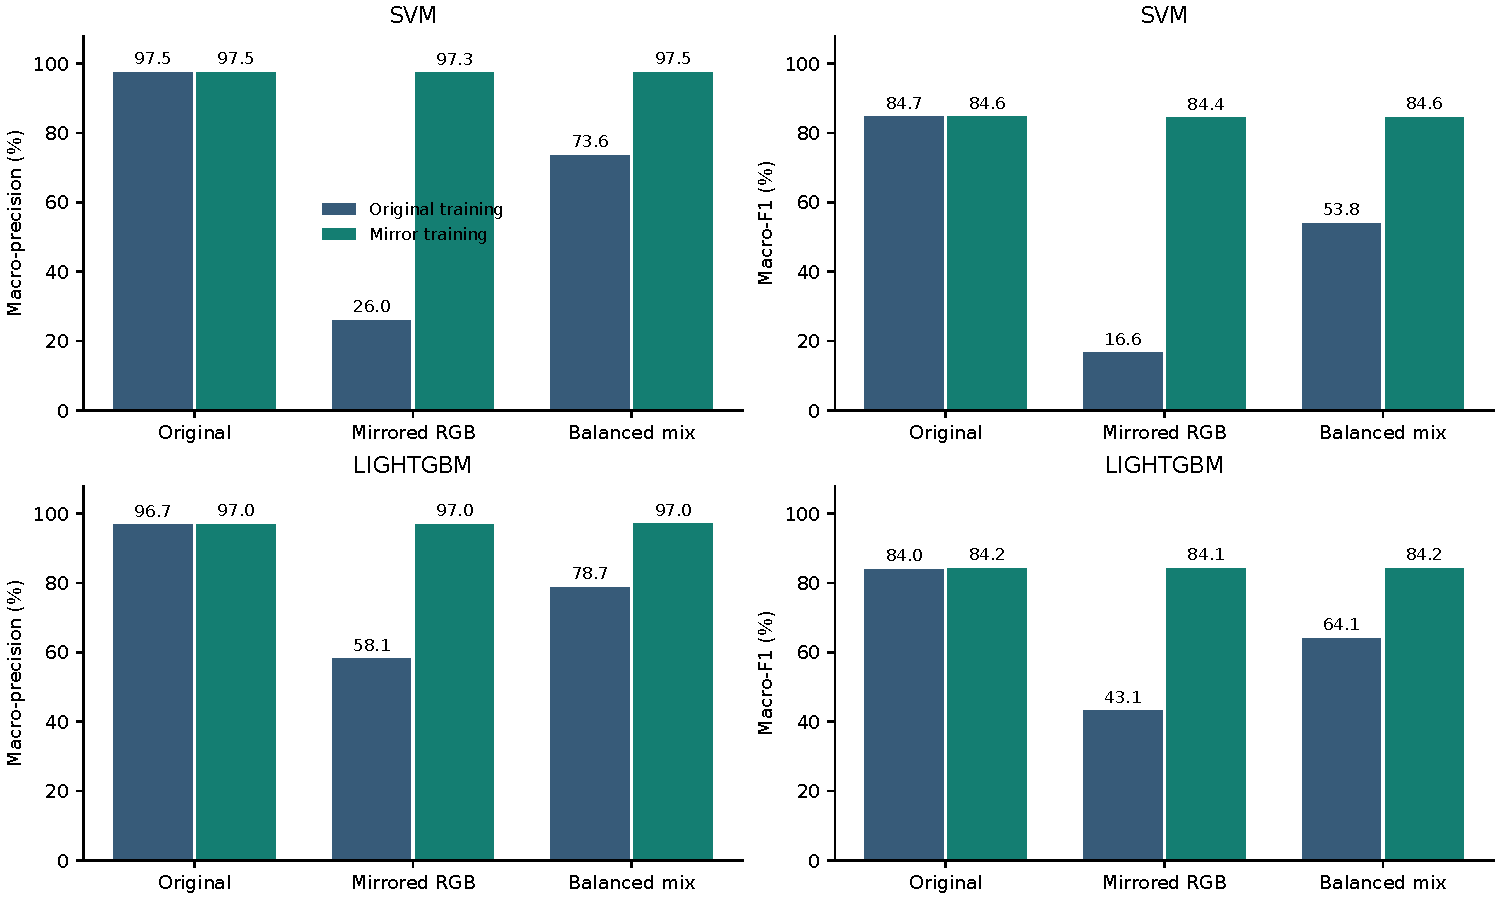
\includegraphics[width=.9\linewidth]{figures/mirror_metrics.pdf}
\caption{Precision and F1 for the two training arms on the three fixed presentations. All attempted sources are retained, including detection failures.}
\end{figure}

\subsection{Reproducibility and Live Comparison}
The supplement \texttt{results/mirror\_01/} stores the extraction/training protocols, source test mix, all fold and per-letter metrics, detection counts, paired changes, confusion matrices with a no-prediction column, and every held-out prediction. Local checkpoints retain pixels' checksums, source groups, both landmark sets, detector labels and features. \texttt{verify\_mirror.py} recomputes metrics and checks source separation, fitting-only preprocessing and model replay. \texttt{report\_mirror.py} generates paper numbers and tables from stored results. Commands are in \texttt{REPRODUCE.md}. These checks establish computational consistency, not independent linguistic validation.

The native live tool exposes a fresh original-only SVM and a mirror-trained SVM as separate comparison models. Both use the unchanged 835-input live encoder. Their deployment fits use all accepted original sources; their cross-validation scores describe the recipe, not an independent test of those final fitted artifacts. The earlier models remain available. A new prospective collection with both hands, hidden predictions, fixed tasks and participant/session separation is needed to test real left-hand performance.
